\chapter{Model framework \label{chapter:modelfw}}

\section{Model framework: introduction \label{sec:frameworkintro}}

This chapter has two aims:

\begin{itemize}
	\item Explain the logical structure of the model framework used in Chapter \ref{chapter:models};
	\item Explain how model `scenarios' are coded, described and presented.
\end{itemize}

The model framework uses the economic and spatial ideas from chapters \ref{chapter:location} and \ref{chapter:spaceconceptsintro} and provides a structure for agents using them to interact. It is built using object-oriented programming, as discussed in section \ref{sec:abmiswhat}. Table \ref{tab:keytable} gives a key for the diagrams used to describe the logic of the model; these diagrams use the code relations between objects to do this. (Appendix \ref{apx:modelcodeoverview} describes the code more traditionally, using UML, and explains the code in more detail.) The rationale for this approach is to present the object structure and the logic of the algorithms in one diagram as clearly as possible, but they should be used in conjunction with the text description. One coding norm that will be used here is to capitalise objects, when they are being discussed as objects. For instance, `Good' is a particular object, distinct from goods generally. 

\subsection{Chapter overview}

The chapter covers the following topics:

\begin{itemize}
	\item The next section describes the three elements that form the foundation for the model framework: actor setup, decision structure and actor data - these are outlined briefly and then discussed in more detail below
	\item The units used in the model are explained
	\item The model `scenario' description method is outlined
	\item The chapter ends with a discussion and critique
\end{itemize}

%\input{ChapterFramework/Tables/keyTable}

%%%%%%%%%%%%%%%%%
% Key table
%%%%%%%%%%%%%%%%%
%http://texblog.net/help/latex/ltx-68.html
\renewcommand{\arraystretch}{1.2}
\begin{table}[!hbt]
\begin{center}

%\begin{tabular*}{0.8\textwidth}{|l|l|}
\begin{tabular}{|l|l|}
\hline 
\textbf{Element} & \textbf{Description}\\
\hline
\raisebox{-3mm}{
\includegraphics[height=6mm]{ChapterFramework/figures/keybits/actorobj.jpg}} & People or firms\\
\hline
\raisebox{-3mm}{
\includegraphics[height=6mm]{ChapterFramework/figures/keybits/nonactorobj.jpg}} & Any other object used in the framework\\
\hline
\raisebox{-3mm}{
\includegraphics[height=6mm]{ChapterFramework/figures/keybits/variable.jpg}} & Grey boxes indicate variables.\\
%\raisebox{-3mm}{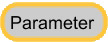
\includegraphics[height=6mm]{ChapterFramework/figures/keybits/parameter.jpg}} & Parameters are fixed for model runs but may change between them\\
%\raisebox{-3mm}{
\includegraphics[height=6mm]{ChapterFramework/figures/keybits/constant.jpg}} & Constants do not change\\
\hline
\raisebox{-3mm}{
\includegraphics[height=6mm]{ChapterFramework/figures/keybits/objarray.jpg}} & An array, or set, of objects, such as the set of all firms\\
\hline
\raisebox{-3mm}{
\includegraphics[height=6mm]{ChapterFramework/figures/keybits/ref2obj.jpg}} & For example, a Person may want to keep a reference to their preferred employer\\
\hline
\raisebox{-3mm}{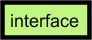
\includegraphics[height=6mm]{ChapterFramework/figures/keybits/interface.jpg}} & A way to provide shared methods to different objects; not important for\\
&understanding model logic, but worth noting where present\\
\hline
\raisebox{-3mm}{
\includegraphics[height=6mm]{ChapterFramework/figures/keybits/method.jpg}} & An object method for achieving a particular model aim\\
\hline
\raisebox{-3mm}{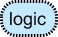
\includegraphics[height=6mm]{ChapterFramework/figures/keybits/logic.jpg}} & Can be one of three things: a logical decision, a calculation\\
& Or an operation on a set (array)\\
\hline

\end{tabular}

\caption{Key for model diagrams \label{tab:keytable}}
\end{center}
\end{table}

\section{Elements of the model \label{sec:elementsmodel}}

\subsection{Two actor setups \label{sec:frameworkActorSetup}}

The framework uses two distinct `Actor' setups:

\begin{itemize}
	\item Single `Actor' type only, interacting with others
	\item Two actor types: `People' and 'Firms'.
\end{itemize}

The majority of the model scenarios are used for testing the economic ideas are working properly, and for this the `People and Firm' setup is used, so that Firms can work as static sources of supply and People as utility-maximisers. The single actor setup, used less often, has no distinction between different types of Actor. 

\subsection{Decision structures and model timeline \label{sec:frameworkDecisionStructures}}

\begin{figure}[h!]
\centering
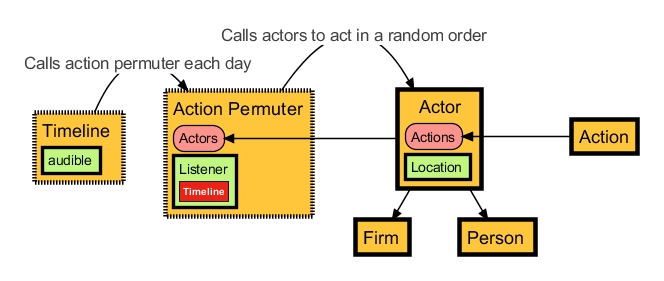
\includegraphics[width=0.75\columnwidth]{ChapterFramework/figures/TimelineActions}
%\includegraphics[width=0.85\columnwidth]{ChapterModels/Figures/hillclimbExcel}
\caption{Timeline sequence \label{fig:frameworkTimeline}}
\end{figure}

The timing structure shown in figure \ref{fig:frameworkTimeline} is very simple: as each day passes on the `Timeline', an `Action Permuter' calls Actors in a given order.\footnote{The Timeline is part of an Observer framework used by other model elements like visualisation and data writing; again, see the code appendix for more details.} The issues around exact ordering are discussed in section \ref{sec:randomisation}. When an Actor is called, they decide what action to take. Actors' decisions can use any of the following:

\begin{itemize}
	\item Instant: act on information collected `now'
	\item Feedback: Act, wait, respond
\end{itemize}

As discussed in section \ref{sec:blindvsrational}, actors take decisions either instantaneously or using feedback from their actions over one or more timesteps. In instant decisions, when actors are called to act, they immediately gather the information they need and optimise based on that. For multi-timestep decisions, actors try an action and then check later whether the outcome was desirable or not before taking their next action. No attempt is made to simulate synchronous decision-making. At the point where an actor is deciding, all others are currently static.

Outside of the Timeline-driven decision structure, there is a third type of `reflex' decision that Actors can take. Here, an Actor is coded to react to requests from other Actors, rather than the Timeline - for instance when a purchase takes place. These reflex actions are mostly just the exchange of stock or money, but can also involve adjusting prices in a `granular' way, rather than the Actor waiting for their decision turn. For instance, this is used in the model in section \ref{sec:prodtowelfare} where granular price-changes are used to equilibriate stock levels.

\subsection{Two actor data sources}

Actor decisions will be based on one or both of the following sources of information:

\begin{itemize}
	\item Internal Actor data, changed by other actors since last a decision was taken. (Example: Firm net income.)
	\item Externally collected data (Example: list of good prices from surrounding Firms.)
\end{itemize}

Externally collected data can come only from other Actors. This is acquired by searching space for a list of all appropriate Actors and forming a set from it.

These three elements - Actor setup, decision structure and Actor data - form the foundation for the model framework. Because all actors face a static world at the point where they decide, their actions can be logically described separately: section \ref{sec:actorSetup} explains how they are put together. 

\subsection{Model units \label{sec:modelunits}}
%\subsection{Model variables and keeping them normalised in an abstract setting}
%\subsection{Use of space}
%\subsection{Space costs 1: good cost method...\label{sec:spacecost1}}

The model framework is abstract: the purpose of specific values for variables, then, is always relative to other values in the model itself, not any external quantity. Because of this, it is always best as far as possible to normalise the values used in order to keep the analysis as simple and clear as possible. Where appropriate, this will mean just using unity (a value of one). This section describes the values used, explains how they are normalised, and how they will appear in the model data presentation.

Section \ref{sec:spaceterms} explained that both one-dimensional and two-dimensional spaces are used, and are referred to as $R^1$ and $R^2$. The size of both $R^1$ and $R^2$ is kept to one number: in $R^2$, width and height are always kept the same. Model space is measured in very small units: a width of one or two is usually used. In some model runs, the distance actors can `reach' is increased. In these cases, world dimensions are defined so that the maximum reach keeps within the boundaries just described for discontinuous space.

\subsubsection{Economic variables}

For `Firm and People' models, the two key economic variables are wage and good price. These both need setting in proportion to each other, as the real wage is actually purchasing power (`how much I can buy with my wage') not the nominal model value. (As discussed below, however, the real yardstick for the model is the amount of utility actors can get for their input.) This is most obvious when using the Engel function as People's utility: the price ratio of wage to goods will determine whether any demand exists for the luxury good. For example, if $\gamma=1$ in the Engel function utility equation \eqref{eq:engelsmurata} and wages and goods are both one, only necessity goods will be demanded (with some tiny quantity of random luxury buying if there is noise, see section \ref{sec:engeltest}). If a unit of wage is higher than the unit price of the necessity good, however, demand for luxury goods will kick in. Since it is this ratio that is key, not the nominal value, model wage values will always start at one and other values changed if necessary.

Some values represent excludable, rivalrous values, where only one actor can `have' them. Both stock and money can come into this category, but note that in a particular model `scenario' (see below), the `flow' of these values may be turned off. 
%For example, if the wage and goods prices are both fixed, money flow may also be turned off.

Since each Person has one day to spend, the number of People determines the total amount of available labour in any model scenario. In models where People are also spending that day on movement, there is thus a zero-sum relationship between time contributed to production versus space.


\section{Actor setup \label{sec:actorSetup}}

\subsection{How People act \label{sec:howPeopleAct}}

\begin{figure}[h!]%
\centering
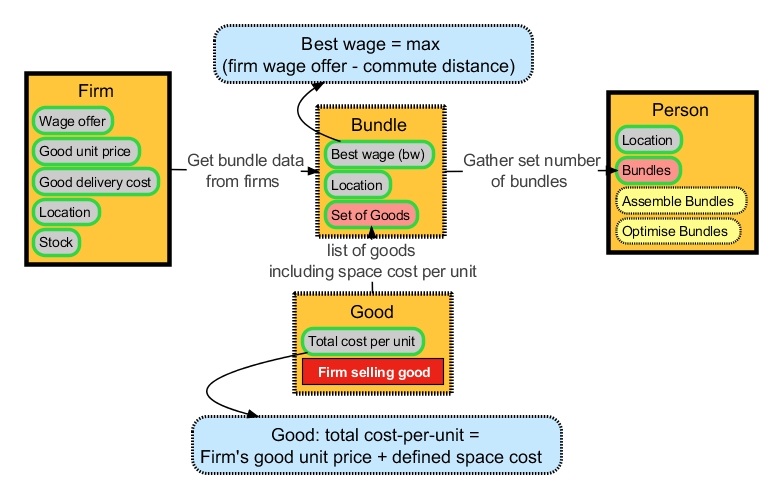
\includegraphics[width=0.95\columnwidth]{ChapterFramework/figures/PersonAction1}%
%\includegraphics[width=0.85\columnwidth]{ChapterModels/Figures/hillclimbExcel}%
\caption{Elements for the Person action}%
\label{fig:personlogic1}%
\end{figure}

%\subsection{How do People turn time into utility? \label{sec:turntimetoutil}}
People have `one day per day' to spend and, as section \ref{sec:keyconcepts_coremodel} pointed out, their fundamental question is, `what is the maximum utility I can get for my time?' Depending on the modelled scenario, this time can be spent on moving through space, on production in their own backyard, and/or put into firms or collaborators in exchange for either goods or money. The description here deals with the most complex of these: people working for money and then spending it on goods. 

People compare a number of `Bundles'. Each Bundle consists of a location, a best wage offer and a list of goods that the wage can be used to buy. They then choose the one that will give them the highest utility. No storage of wage between iterations is allowed: the wage must be spent or lost on each turn. 

%How exactly does this happen? There are two elements:
%\begin{itemize}
%	\item Bundles are assembled.
%	\item Bundles are optimised to turn People's time into the best possible utility.
%\end{itemize}

Figures \ref{fig:personlogic1} and \ref{fig:personoptfr1} outline what happens when a Person is called to act. An `instant' decision is made on what to buy, who to work for and where to locate based on data they gather when it is their turn. Figure \ref{fig:personlogic1} shows all the elements prior to utility maximisation. As well as their set of Bundles, People have two methods: `assemble Bundles' and `optimise Bundles'. The next section (and figure \ref{fig:personoptfr1}) describe this last step in more detail. An overview of the methods involved is as follows: 
%\cmt{in a situation where there are firms. How/where to describe other scenarios? Get this one done first, then think about it.} 

\begin{itemize}
	\item Method `assemble Bundles': assemble a series of Bundles; one from my current location, and a defined number from other random locations.
%	 A single Bundle is put together as follows:		
\item Method `optimise Bundles': two steps. 
\begin{itemize}
	\item Optimise each bundle's mix of goods to get a single utility value
	\item Select the Bundle with the best utility: accept the wage, pay for goods and, if applicable, move to the new location.
\end{itemize}
\end{itemize}


\subsubsection{Assembling Bundles}

As outlined in figure \ref{fig:personlogic1}, a Bundle consists of the following: 

\begin{itemize}
	\item The centre location of the Bundle. One of these will centre on the Person's current location. Others are given random locations within a defined range. The rationale here is this: each separate Bundle allows a Person to ask, `if I were to move to that spot, would I get a better utility value?'
	\item A set of Goods, where each Good is an object containing the good's total cost per unit (including delivery cost) and a reference to the Firm selling the good. That reference provides a way to buy goods and get a wage if the Bundle is selected.
	\item A `best wage' selected from a set of Firms and taking account of commute cost.
\end{itemize}

Each of these is dealt with next, but here are a few preliminaries. Firstly, What determines the number of random bundles? The value is arbitrary: the higher it is, the more likely on any one turn that a person will find the `best' utility option for them. Over a number of days, however, this will tend to happen anyway. Section \ref{sec:timingstr} goes into the issue in more depth: what difference do timing structures make for outcomes? The range for a Bundle's centre location can also vary. It may be limited by one day's distance, weighted towards closer distances, or People may be given free choice over the whole model space.

The first step for a person getting Bundle data is to get two lists of Firms: one for finding the best wage, another for a full list of available goods. Two sets are required since distance to potential employers may be restricted by commute distance, whereas good delivery can occur from further afield.


\subsubsection{Selecting the best wage \label{sec:wageselect}}

How does the actor decide who to contribute to? The simplest method allows them to know exactly which option will give them the highest utility and select accordingly. This is not always directly possible, for reasons discussed below. The next simplest is to use price: they choose the highest price on offer for their input, or using a function like the \gls{ces}, they can buy a utility-maximising mix of available outputs. Section \ref{sec:prodtowelfare} presents a model of this type, where the more challenging problem of using price to signal between production and welfare is discussed. 

Each Bundle has one unique `best wage' offer. Selecting this is a two-step process: first, gather a set of all Firms within commute distance. Second, select the Firm offering the best wage, accounting for commute distance from the Bundle's location centre. This best wage can be described as follows. Let $F=\{f_{1},f_{2},...,f_{n}\}$ be the set of Firm objects. Each Firm has a wage offer, which is `the amount paid for one day's input'. For each $f\in F$, $W_{f}$ is that wage offer. To describe space cost, the distance in \emph{time} can be used: for each $f\in F$, $t_{fa}$ is the time taken to travel between $f$ and $a$. 

Let $l_{af}$ be the labour available to contribute to $f$ by Person $a$. The amount of labour they have available for contributing is just their own time (one day, $t_{a}=1$) minus commute time. Here, a `commute' is taken to be twice $t_{af}$. The upper distance limit on whether a firm enters into $a$'s considerations has to be less than $a$'s one available day in total - half a day there, half back - otherwise there is no time left at all to contribute to production. So $f$ can only be a maximum of half a day away. Given all this -

\[
l_{af}=t_{a}-2\cdot t_{af},\; 0<l_{a}<1\]

If $W_f$ is $f$'s wage for a full day, and $a$ has $l_{af}$ to contribute (a fraction of their full day), this means the wage they will get is just $W_{f}\cdot l_{af}$. The best wage for Person $p$ can now be defined as:

\begin{equation}
bw_p=max\; \{W_{f}\cdot l_{af}\mid W_{f}\in F,\; t_{af}<0.5\}\label{eq:bwpmax}
\end{equation}

So, the best wage for Person $a$ is the maximum value from the following set: all wage offers proportionate to Person $a$'s labour input from those firms in $F$ who are less than half a day away.


\subsubsection{Optimising bundles \label{sec:optimisingbundles}}

Once a Bundle is assembled, it can be passed to the Person's optimisation routine.\footnote{As appendix \ref{apx:modelcodeoverview} explains, there is only one actual, static Optimiser class, but in terms of a `functional mapping'  it can be considered internal to each Person.} This produces a utility level from one of two possible utility-maximising methods, and the result is stored in the Bundle. Finally, the Bundle with the maximum utility level is selected: the wage offer is accepted and the optimal quantity of goods is bought.

%Section \ref{sec:frameworkUtility} goes into the full details of how this happens.
The logical goal is simple: for each Bundle, find out how to spend the best wage on the set of Goods as optimally as possible (without actually spending it) then choose the optimal Bundle. Figure \ref{fig:personoptfr1} is an overview of the process. Assuming the Person has the set of Bundles they will optimise, the sequence is as follows. 

\begin{figure}[h!]%
\centering
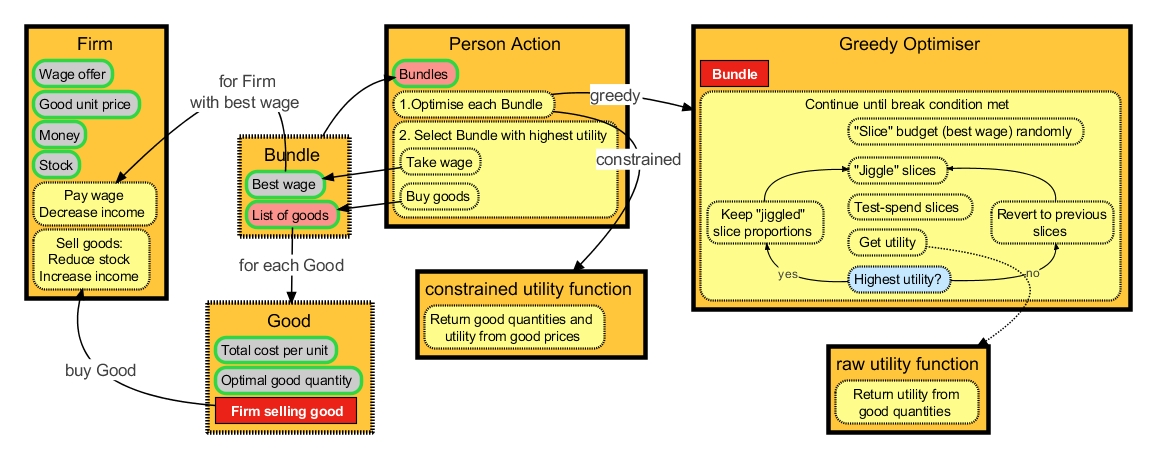
\includegraphics[width=1\columnwidth]{ChapterFramework/figures/PersonOpt2}%
%\includegraphics[width=0.85\columnwidth]{ChapterModels/Figures/hillclimbExcel}%
\caption{Optimisation of Bundles in a Person's action}%
\label{fig:personoptfr1}%
\end{figure}

\begin{itemize}
	\item Optimise each Bundle. This happens in one of two ways:
	\begin{itemize}
	\item $(1)$ A `greedy optimiser' uses the following method - 
\begin{itemize}
\item The greedy optimiser iterates for a set number 
	\item The iteration is initialised by randomly slicing the budget (the best wage), one slice for each Good in the bundle, before beginning the iterations, so that each has a starting guess price. The iterations are:
	\item `Jiggle' the slices, changing their proportionate size slightly.
	\item `Test-spend' those slices on each Good: find out how much could be bought with the current budget slices using the per-unit price for the Good.
	\item Get a utility level for these quantities of goods. The Utility function is logically separate: the Optimiser deals only with this process of random slicing and adjusting.
	\item If the utility level found is the highest so far, keep the current proportion of slices and return to the 'jiggle' point. Else, revert to the previous slice proportions and try again. This has the effect of ratchetting the budget slices (and thus the spend per Good) towards an optimum.
\end{itemize}
	\item $(2)$ `Constrained' optimiser: a Bundle is passed directly to a code version of the constrained utility optima described in section \ref{sec:constrained}.
	\begin{itemize}
	\item{The Good prices and budget are used to directly calculate optimal good amounts. The utility level is then `read back' from those amounts.}
	\end{itemize}
	\end{itemize}
	\item Once each Bundle has an optimum utility, select the Bundle with the highest utility, then:
	\begin{itemize}
	\item Take the best wage: this instructs the Firm to pay the Person.
	\item Buy goods in the quantities found optimal by this Bundle.
	\end{itemize}
\end{itemize}

Figure \ref{fig:CESHillClimbIllustration} graphs data from the greedy algorthim in action. A bundle containing sixteen goods of equal cost is optimised for a CES function over a thousand iterations. (The optimum for a CES function with equal-value goods is  already known from section \ref{sec:CESbasics}: an even mix.) In this example, the optimum is found quite slowly: this helps to illustrate the process. The first graph shows initially random budget split guesses converging on the optimum mix of $0.06$ for each good. The second shows the marginal utility gain from each iteration; most of the gains happen very quickly, after which almost no extra benefit accrues (though there is a very small amount of further convergence.)

%The important difference to analytic constrained optimisation is that people can work with any number and type of good and can deal with limited stock levels. If People find an optimal amount simply isn't available to them, they must spend their wage accordingly. 
%In contrast, a standard constrained optimisation results in an `objective' optimum (see \ref{sec:produtility_agents}). In this model framework, people may find that this optimal amount simply isn't available to them, so they must spend their wage accordingly. As well as being able to deal with any quantity of available good, this approach also allows easy swapping of utility 

\begin{figure}[h!]
\centering
\includegraphics[width=0.85\columnwidth]{ChapterModels/Figures/hillclimbExcel}%
\caption{Utility-maximising stochastic search algorithm, optimising a CES function with 16 goods over a thousand iterations (x axis)}%
\label{fig:CESHillClimbIllustration}%
\end{figure}


\subsubsection{Overview of People's utility \label{sec:frameworkUtility}}

%Things to do here:
%Give a run-down of the actual utility details and how it fits together
%Give a run-down of the structure of the optimisation

The technical detail of optimising utility has just been covered. There are three further points worth covering briefly.

People have utility functions based on those described in section \ref{sec:econconceptsintro}. In any one model run, all actors have identical tastes: they all use the same utility function. One useful assumption from using identical tastes is that, in one-good models, only the absolute quantity of that good matters. This is because the same quantity of good will always return the same utility for each Person, regardless of the form of utility. For example, if all people have an identical one-good utility function that happens to have \gls{increts}, the \gls{increts} will just produce the same level of utility for everyone, given the same good input. In contrast, if tastes were not identical, one Person could gain more utility from the same quantity of good as another. Many of the simplest model tests use the assumption that a single good quantity can stand in for utility.

In all situations where more than one good is available, People use utility functions. The form of utility used must also imply the production structure, though not the actual production function itself. For instance, a two-good utility function means a model where only two goods are made, though many firms may compete to sell each good. An $n$-good utility scenario, using the \gls{ces} function, will have each Firm making one unique good, as they do in \gls{monocomp} models.

Actors using this method are rational in only the most basic way: they are able to judge when one Bundle is better than another. This rationality reflects basic micro-economic preference assumptions. Bundles of goods are `complete': any two bundles can be compared. They are also transitive: as Varian puts it, ``if the consumer thinks that $X$ is at least as good as $Y$ and that $Y$ is at least as good as Z, then the consumer thinks that X is at least as good as Z'' (\citealt{varian_intermediate_2006} p.35). 

%Why take this approach, when it is possible to produce constrained optima that include price? 
%MM1 20pp/23	Reasoning behind bundle approach; cf. to Fowler's 'objective demand' approach. Write up.

%again, I'm not sure where to discuss the hill-climb, the black-box nature of it, compared to some `online' approach. At the moment, I haven't used the online approach, so I'll leave it. Needs discussing somewhere.



\subsection{How Firms act \label{sec:howFirmsAct}}

In many of the partial models, Firms take no actions at all: they serve as points of good supply only. Where they do take actions, the method used is as follows. A Firm's decision process is based on feedback between timesteps. A firm takes an action, waits, and then responds depending on how its own internal data has changed (see figure \ref{fig:FirmAct1}). Because of this, the structure of Firm decision-making is quite a lot easier to describe, since Firms do not collect any data externally themselves. 

At time $t-1$, a firm chooses one of either location, good unit cost or wage offer, and `jiggles' it, altering it slightly in a random direction. It remembers these choices. At time $t$ the firm asks, `did my net income between timesteps increase?' If yes, it repeats the previous action (hence needing to remember what it was), with the possible addition of increasing the size of the adjustment. If not, the Firm returns to its initial random search.

\begin{figure}[h!]%
\centering
\includegraphics[width=0.85\columnwidth]{ChapterFramework/Figures/FirmAct1}%
\caption{A Firm's feedback mechanism: ``jiggle'' a random value, wait to see effect.}%
\label{fig:FirmAct1}%
\end{figure}

The result is that, through blind search, Firms are constantly searching for ways to improve their net income. Note that this method disconnects them even further from any analytic approach to optimising. Where at least People do use a utility function (albeit one that calculates utility solely from raw good amounts), here the firm does not directly consider its own input or output requirements. Also, while they act on how their own internal data changes, Firms know nothing about how those changes occur. 

%\subsubsection{Firms' production functions}
%\cmt{This is all described in chapters 2 and 4. What do I want to say here? Something specific? It only counts for the one model so far. Uhmmm.}
%The simplest Firm production function turns a given amount of labour input into good output. For a given time period, how can this be worked out? Section \ref{sec:dmr} explored the problems of getting agents to utilise \gls{increts} in an agent-based time structure. The goal is to allow the model's Firms to gain from those \gls{increts}: output per unit of input labour should increase as the total labour contribution rises. The problem is finding an effective way to allow that total labour quantity to change, given the discrete, asynchronous nature of decision-making.
%The solution used is as follows. Two things happen: first, when a Person chooses an employer, they receive their wage on the spot, and their contribution to the Firm's production is calculated then and there. However, they `leave' a record of their contributed time with their chosen employer until it is their turn to act again, when they remove it and decide anew. This means that, when anyone else comes to contribute, that time is still considered as an input, as far as the production function is concerned. This allows \gls{increts} to occur. This approach is discussed in more depth in section \ref{sec:backyard} to see exactly what impact its assumptions have on model outcome.

\section{How the single-actor models work \label{sec:singleactorFramework}}
%\cmt{single actor models plural? Plus, should the lov eos stuff be in econs?}

Using a single actor-type does away with many of the complications that come with modelling the interaction between Firms and People. Most importantly, single-actor People need only seek to directly improve the utility they can get for their time. There is no intermediate stage where money is required for wages or good purchase.

Section \ref{sec:marketstructnspace} outlined how, theoretically, \gls{increts} are required to make trade possible across any distance. The two forms of \gls{increts} that can give Actors the ability to find better-than-backyard options are \gls{eos} and \gls{lov}. Section \ref{sec:singleActorLoVAnalytic} presents an analytic argument to show that single actors can indeed find trade across space worthwhile, even with \gls{lov} alone. However, the single-Actor agent models do not necessarily require People to be comparing backyard production to trade in the same way, presuming instead that they will always trade. 

%In these scenarios, Actors always have the option of simply producing in their backyard. This gives a base for comparison: one day's input will always return one unit of utility. For anything spatially interesting to happen, then, Actors must be able to find outcomes that can better this backyard situation: utility must be more than one.

On the face of it, \gls{eos} and \gls{lov} produce higher utility in very different ways. \Gls{eos} stem from a more-than-linear increase in output for a given input into production, whereas \gls{lov} is a purely utility-based function. Mathematically, however, output from both \emph{can} appear identical. \Gls{eos} does not need to be a physical output increase; it can be an increase in the value of each unit. If this was the case, physical weight per unit of value (value density) could increase \emph{or} decrease.

Another difference, one might argue, is that \gls{eos} implies an indivisibility. In the case of labour, workers must come together at a particular site to produce the goods. Again, however, \gls{lov} can be said to require the same: there must be a `point of trade' for the exchange of goods and, even if they are not consumed at that point, the future utility-increasing consumption is implied in the exchange's successful outcome - otherwise it would not have taken place.

\section{Model `scenario' setup \label{sec:scenarioFramework}}

Individual model `scenarios' will examine a particular aspect of the thesis issues. For each scenario, the main components will be described in table form as succinctly as possible. Where a scenario has particular idiosyncracies, these will be described below the model scenario table. 

\subsection{Model scenario description method}

The \emph{components} of model scenarios vary in a limited number of ways: table \ref{tab:components} lists these commonalities, and the following discussion explains the table entries in detail. 

\input{ChapterModels/Tables/modelComponentsTable}

\subsubsection{Run type}

Model iterations are considered `days'. A model run will last a given number of days. Generally, all actors will take an action at least once a day (with some exceptions where firms only respond every few days.) The particular number of days chosen will vary depending on the appropriate amount of time needed to find a useful result. 

In each scenario, a single model run will be used to illustrate the basic point. Subsequently, parameter sweep runs may be used. These repeat model runs, while altering a particular parameter. See the discussion of parameters below for a consistent way of describing how they change.

\subsubsection{Actor type}

As outlined in section \ref{sec:frameworkintro}, Actors will be either of two types, Firms and People, or a single type (just referred to as `People'). 
%The distinction between actor types may be hard-coded, or where there is only one type of actor, differences between them may arise through interaction. For example, the `backyard' model scenario in section \ref{sec:backyard} uses one actor type, where each independently decides who to collaborate with.

\subsubsection{Actor number}

The number of each type of Actor in a particular scenario can be set specifically, or given as a quantity per unit distance or radius, so that the total amount stays consistent regardless of the size of space used. Reasons for a chosen number will be given. The general principle is to use as small a number as possible to achieve useful insights. In situations where agent number affects outcomes in important ways, the total may be changed over a parameter sweep run. See also the discussion in section \ref{sec:agentnumbers} on the use and meaning of agent number.

\subsubsection{Actor action}

A basic description of the actions to be taken will be given for each scenario. Some are more common than others: people looking for the best wage and goods prices; firms changing cost settings in search of better net incomes. Action types are usually intuitive and obvious. 

\subsubsection{Timing}

Section \ref{sec:timingstr} explained the issues around timing. Scenario tables will summarise as briefly as possible what particular structure is being used for a scenario. 

\subsubsection{Space type}

As described in section \ref{sec:spaceterms}.

\subsubsection{Actor location}

This describes both Actors' initial location starting conditions, and their relation to location change. Location may be randomised to start with either over the whole defined model space or within a certain distance or radius, or they may be set to a particular pattern, most often a line or circle (which stands in for a square or triangle if four or three actors are used.) Actors will also either be permanently fixed at this initial locations, or able to move. 
%If mobile, their movement may a `crawl' or a `jump' - that is, they will move short distances from their current location, or will be able to move anywhere within a defined range. Lastly, these movements may cost them. This comes under the broader heading of space costs.

\subsubsection{Space costs}

A model scenario will state whether space costs are used, and how they are implemented. 
%As well as any costs incurred through actor movement, two other types of space cost may be used: good delivery cost and land cost. \cmt{may also include land costs e.g. via landlord agents, but don't know if I'm including this in the write-up yet.}

\subsubsection{Values}

The nature of the values used in a model scenario will be described. Table \ref{tab:keytable} explained the distinction made between variables, parameters and constants as regards each model. Of most importance will be those values set as constants for any particular scenario. For example, wages may be fixed and stock unlimited.


\section{Framework discussion \label{sec:nutsnbolts}} 

\subsection{Interdependence of decision structures \label{sec:decstruct}}

It is not easy to meet the \gls{oop} ideal of fully encapsulated, autonomous agents in an economic modelling scenario. Indeed, it could be argued that in an economic modelling situation, it is not desirable. Much of the agent literature seems to have absorbed a modelling paradigm required for `instrumental' agents able to carry out real-world tasks. For example, Wooldridge's `Introduction to Multi-agent Systems' mentioned in chapter \ref{chapter:ABM} is imbued with this sense of the need for autonomous agents,  where ``each agent is assumed to have at least one thread of control'' (\citealt{wooldridge_introduction_2009}). 

Putting aside reasons of computational expense, programming fully autonomous economic agents in this way is a massive task. This becomes particularly apparent when trying to construct the timing framework. The ideal of fully independent objects mediating their interaction with a separately threaded environment is a stark contrast to the reality of the interdependence of different actor decisions. This section looks at a number of examples of this that arose during model development, and includes references to results in chapter \ref{chapter:models} that examine these problems more closely.

Any decision which will, in the process of optimising, interact with other actors' decisions can be considered `online'. In contrast, an actor able to optimise a utility function without affecting the basis for its optimisation is `offline'. The terminology is Holland's: Mitchell describes its use in the `two-armed bandit' game, where the player tries to discover each arm's mean payoff and variance:

\begin{quote}
``... the goal is not merely to guess which arm has a higher payoff rate, but to maximise payoff in the course of gaining information through samples to the two arms.'' (\citealt{mitchell_introduction_1998} p.119 discussing \citealt{holland_adaptation_1975})
\end{quote}

The difference between off- and online decision-making is partially blurred with many agents, and depends on timing structures. For the two main types of decision described in section \ref{sec:frameworkDecisionStructures}, `instant' is partly offline, since Actors face a static world and can select the objectively best Bundle. It is also partly online, in that the global optimum is affected by the number of random Bundle locations they can test at any one time; the movement towards a global optimum is thus not instantaneous, and Actor choices interact. This can lead to path-dependence for single Actors, but the global outcomes are consistent; see section \ref{sec:spatialeq}. The `feedback' decision process actually relies on being `online' since the Actor requires the `world' to respond to its action to know what to try next. This is discussed in-depth in section \ref{sec:dmr}.


\subsection{Communicating costs \label{sec:comm_costs}}

Agent models proceed over many iterations. In a spatial economic model involving goods, this presents two immediate problems that need solving. Firstly, in such a world, what moves between economic linkages each timestep: actual resources, where actors actually `exchange' some excludable, rivalrous quantity? A common way to avoid this is to presume goods perish before the next timestep (e.g. Tesfatsion's `hash and beans' model; {\citealt{tesfatsion_agent-based_2006} p.848). In the thesis model, where good stock is not fixed, the presumption of both persistent and perishable stock are tested to see the effect on the link between production and welfare (see section \ref{sec:prodtowelfare}).

Things become more complicated with money, however. Actors need some method for communicating costs to others. Again, for the partial models in chapter \ref{chapter:models}, it is easy enough to assume that, while actors need to use prices, that does not always need to imply money is exchanged. This is a parallel assumption to perishable stock: Firms set prices, and wish to maximise income on a given iteration, but the money they receive `perishes' immediately. This avoids the huge complications of making money flow function: any simple attempt to implement money exchange as `actual resources' immediately finds that moneyflow dynamics themselves loom over other model problems. 

Figure \ref{fig:simplemoneytest} illustrates the basic problem for a set of zero-intelligence agents running for 200,000 iterations. One hundred agents are given an initial one hundred in currency. They then select another actor to give a unit of currency to, if they have any. The consistently stable result is a bounded random walk resulting in a large inequality\footnote{There is a comparison here to Epstein's take on Schelling from section \ref{sec:generative}. This model `grows' an uneven distribution of wealth with a gini coefficient not too far from the reality of many countries. Does it explain it? There is not a large gap between claiming it does to making justifications for wealth inequality as a natural, unavoidable consequence of money flow.}. Initial tests using the more economically sophisticated agents of the thesis model suggested that such dynamics could play a large role in outcome. 

\begin{figure}[h!]%
\centering
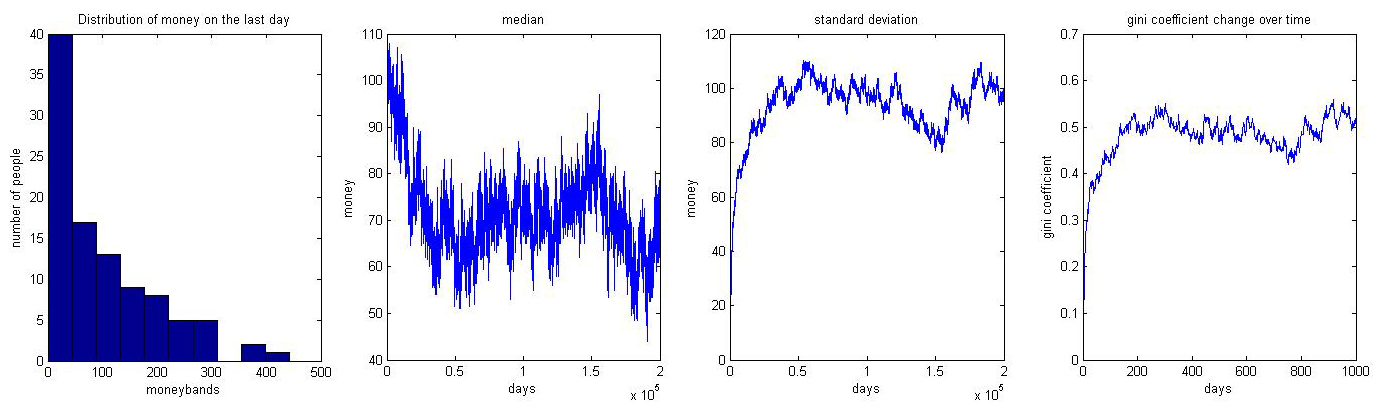
\includegraphics[width=1\columnwidth]{ChapterABM/figures/simplemoneytest}%
\caption{Zero-intelligence agents exchange finite money, beginning with equal amounts. \label{fig:simplemoneytest}}%
\end{figure}

It is a large assumption to exclude further analysis of this dynamic from the model,  since the impact of money flow may be key to interpreting some types of model outcomes. Yet in being strategic about simplifications, this is a useful one to exclude. This is not to say that modelling flows is either unworkable or unimportant: the concluding discussion returns to this point. There are many modelling approaches that could potentially avoid the fate of the zero-intelligence model above, and it is an open question whether more economically sophisticated agents would achieve this, or whether it would require some model implementation of a banking structure forcing actors to `rent' money rather than keep it. (See \citealt{oeffner_agent-based_2008} for an agent-based macro-economic model that attempts to incorporate this kind of `monetary circuit'.)

\gls{ge} (and other economic) models avoid the issue through, firstly, not dealing with flows, and secondly, through using `price' of one good as the `numeraire'. In the case of the \gls{coremodel}, for example, one good is kept to linear production and that sector's worker number is fixed exogenously. This keeps its value constant, so it can work as a unit of comparison.

In an agent context, if some attempt is made to treat money or goods as `actual resources' so they can function as a numeraire, problems immediately present themselves. If, for example, two Firms each make a different good, and one is deemed the numeraire, each must pay wages in it. How does the non-numeraire Firm do this? It must acquire the currency, and can only do this by exchanging what it produces - yet there is no guarantee the numeraire-producers want to exchange. 

The model in section \ref{sec:prodtowelfare} avoids these issues by presuming actors are gifted a quantity of input to spend on each turn, which can be put into either production or movement. It is thus open to interpretation as their time, spent on space or labour. This circumvents the problem of `real' flows and allows comparisons of change, as the basis for the model becomes actors asking, `what quantity of utility can I get for my input?'

An overarching question from this is whether Howitt is right to argue (see section \ref{sec:ace}) that an agent approach ``forces one to make explicit the mechanisms through which individual actions are coordinated, for better or worse'' (\citealt{howitt_coordination_2006} pp.1068). Deciding \emph{which} mechanisms are the focus for a particular model would appear to force quite the opposite: a Friedman-like need to acknowledge which dynamics are excluded or assumed away.

\subsection{Timing structures \label{sec:timingstr}}

Section \ref{sec:mapping} argued that agent models should be designed with functional mapping in mind, not code mapping. Nowhere is this more true than when constructing the timing inter-relations of the model. When should an actor take an action? There are a number of approaches. First, is it required that all actors should take an action on every iteration? This would be the case if, for instance, an actor needs to look for employment and spend their wage on every turn. This is the approach used in this thesis: it allows for non-synchronised action, and so meets with the `no clearing market' condition imposed by space (see section \ref{sec:ace}), but forces all actors to take at least one action per turn. 

Contrast this to another common approach: to require a specific collective goal to be met on each iteration. This is the method used for market-clearing or auction-based systems, and by the \gls{coremodel}'s short-run wage equilibrium calculation. The collective goal is to reach a point where no actor is able to improve their welfare further without making someone else worse off: this is Pareto optimality\footnote{Blaug has a good discussion of this: ``the beauty of Pareto's definition of a welfare maximum was precisely that it defined the optimum as one which meets with unanimous approval because it does not involve conflicting welfare changes''. This ruled out the possibility that one could ``evaluate changes in welfare that do make some people better off but also make other people worse off'' (\citealt{blaug_economic_1997} p.573-4).}. In an analytic context, this collective goal is achieved through equilibrium, built on a mathematical argument about how actors get there (see section \ref{sec:ace}).

In an agent context, stopping conditions could do the same job. In an agent-based clearing market, for example, the iteration may not be over until all Firms have the labour they require, or all People have the wage they want. Note that, in that situation, Firms may end up without having employed all the labour they would prefer, or some People could find themselves unable to work - but if either condition is met, the iteration terminates. This scenario would mean actors may act many times before one of those two stopping conditions is met: they are not limited to a single action each per turn.

\subsection{Randomisation and timing of actions \label{sec:randomisation}}

The model uses a single static `Randoms' class to provide consistent randomisation globally. A random seed provides both exact repeatability and the ability to change the seed for model runs where aggregate results require a full random spread of outcomes.

Randomisation of actors' timing can be used to avoid artifacts arising as a result of actor order (\citealt{gilbert_agent-based_2007} pp.27) but it raises its own problems. Consider a common scenario where the order of all actors' decision points are randomly permuted on each iteration. The probability of getting any particular point in that order is the same for all actors. However, over \emph{two} days, the time between any one actors' actions will vary. The most common outcome is an exact one day gap, since it has the highest possible number of chances to appear from both days' permutation: a one-day gap can fit into a two-day space beginning at any point on the first day, right up to the last slot. If $n$ is the number of actors being permuted, there are the same number of one-day gaps as $n$. Each consecutive length of shorter gap has $n-1$ chances, until at both extremes (with a small but equal probability), two actions will either be consecutive (at the very end of one day and the beginning of another) or nearly two full days apart. The result is a pyramidal distribution. The histogram in figure \ref{fig:permuteGap} confirms this from a model run for actions of ten thousand actors with daily randomly permuted actions, over a thousand days.

\begin{figure}%
\centering
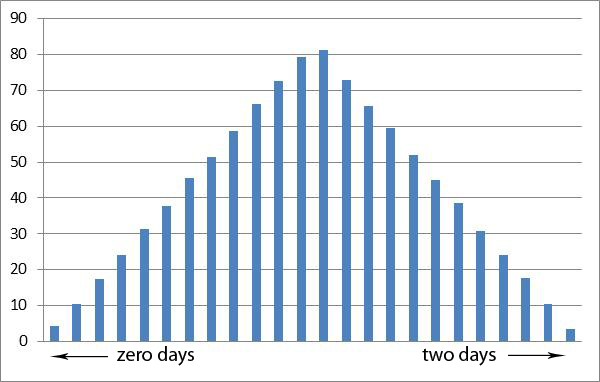
\includegraphics[width=0.5\columnwidth]{ChapterABM/figures/PermuteGapHistogramPSD}%
\caption{Histogram: ten thousand actors over a thousand days, 24 bins, showing how many times on average actors have an action gap between zero and two days, when the order of actions is permuted randomly on each turn.}%
\label{fig:permuteGap}%
\end{figure}

Using a random permutation, then, the time between actions will never be consistent. However, over many iterations, this averages out, so why should this be a problem? It is important to be aware that the above dynamic exists, as it can explain errors in agent decisions that would otherwise remain mysterious. Any decision process based on feedback between $t$ and $t+1$ may be affected. One of these situations is this: a scenario with both Firms and People, where Firms make decisions based on responding to a change in net income between iterations. Any Firm presuming the gap to be a full day will be using faulty data. There are (at least) three ways around this. Firstly, the actions of People and Firms can be put into two `bins' and permuted separately. This guarantees that all People will have made their decisions before Firms come to act. Second, Firms can be allowed to know the length of time between decision points and alter their decision-making (for example, by correcting the rate of change of net income accordingly.) Third, some other method of permuting that damps the variability between timesteps could be used, such as a random walk. This thesis uses the first of these. 

\subsection{Economies of scale and avoiding the need for strategy \label{sec:abmprod}}

As section \ref{sec:prodfuncts} discussed, considered statically, \gls{eos} are entirely straightforward: an equation describes the relationship between the level of input and the given output. But if many actors are deciding whether to input time into a production function, how do they decide? The best choice will in part depend on the levels of output available from Firms - but this is determined by what all other actors have decided. This leads to a catch-22: should an actor wait to see what others do? If everyone does this, how can production get going at all? Once they have made a decision, how is the output itself determined - or more specifically, when, given that both input and output are flows in a multi-timestep situation?

If actors are deciding simultaneously, this can be framed as a game-theoretic problem, solveable for small numbers of actors, but increasingly problematic with larger numbers, and impossible if actors are not synchronised. The choice actors must make in this situation shares something of the dynamic in the ``El Farol Bar problem'' (\citealt{ arthur_inductive_1994}). Everyone makes a decision about going to the bar, but if more than a certain percentage turn up, it is so crowded that no-one is happy. All actors, however, must decide simultaneously. Edmonds describes it thus:

\begin{quote}
``Any model of the problem that is shared by most of the agents is self-defeating. For if most agents predict that the bar will not be too crowded then they will all go and it will be too crowded, and vice versa.'' (\citealt{brenner_modelling_1999} p.12)
\end{quote}

The \gls{eos} problem is the same dynamic in reverse: all actors gathering in one firm will give a \emph{higher} payoff, but there is no way to know who will choose where. The thesis model uses a `granular' approach to avoid these pitfalls. While it has its own issues, it does manage to successfully power the `transmission belt' between production and welfare. This method will be described first, followed by a more detailed discussion of its rationale. The following section (\ref{sec:blindvsrational}) also discusses a more detailed `pseudo-code' thought experiment examining the catch-22 problem.

In the thesis model, when actors decide where to contribute their input, they do so then and there, at the point of decision. They then \emph{leave} their input with whoever received it until their next turn to act. It stays there for one whole `day' (on average, given randomisation of actor order, see section \ref{sec:randomisation}), when it is removed by the same actor prior to re-taking the decision. At the same time, the quantity of output produced is \emph{also} worked out. This is done from the producers rolling record of the quantity of contributed input from all actors. Let the producer's total current contributed input be $T_p$. When an actor adds their input, $t_a$, this rolling record can be used to calculate the output from the actor's contribution, $g_a$:

\begin{equation}
g_a = f(T_p) \cdot (t_a / T_p)
\end{equation}

Here, $f(T_p)$ is the \gls{eos} function, giving a total output figure from all current input. The actor's input divided by the total input, $t_a/T_p$, gives the proportional contribution of that actor. These two can then be multiplied to give $g_a$, the `granular' quantity of extra output produced at that point, which goes into the producer's stock.

What are the problems with this approach? Simply that actors are forced to make optimising decisions given static information: they are robbed of the ability to even attempt to make strategic decisions or develop expectations. Given what has just been said, however, it is the structure of the problem itself that robs them of strategy. The issue here, as Oeffner points out, is the difference between risk and `true uncertainty' (\citealt{oeffner_agent-based_2008} p.25-6). The problems described above represent true uncertainty: probabilistic outcomes are incalculable. As Oeffner points out, actors with `rational expectations' in these situations will do no better than myopic ones. 

Exactly the same issue arises for space-cost decisions in the presence of density costs in section \ref{sec:spatialeq}, though the model in section \ref{sec:firmsLoV} looks at a situation where risk is a component. (The ideas in that model are discussed below in section \ref{sec:dmr}.)

\subsection{Blind versus rational choice: an illustration of the problem with economies of scale \label{sec:blindvsrational}}

This section looks at a small concrete example of the interdependency of decision structures and model `world'. The \gls{coremodel}-style of \gls{increts} \eqref{eq:coremodelMprod} is used, with the fixed labour requirement set to 3. This means that no production is possible at all unless three units of labour are input: an indivisibility. This is straightforward enough to impose analytically, but how might it work in an agent context? 

Consider a scenario where actors choose an employer and goods in the same `moment' (that is, during one action). Assuming that they are completely myopic, zero-intelligence actors, they are unable to make judgements about future timesteps. As a result, they will not work if no goods are available. There is no point: there is nothing to buy. Equally, if no work is available, they cannot \emph{afford} to buy anything. This can lead to a catch-22: if Firms have no stock, they need labour to make more, but no-one will work if no stock is available. Compare these two possibile approaches actors might take in this situation, both of which have arisen as solutions for getting actors trading:

\begin{enumerate}
	\item A `rational choice': actors decide sequentially, looking at what Firms are producing in order to choose whether to work. If no goods are available to buy, there is no point in working.
	\item A 'blind choice': At $t$, actors randomly choose a potential employer. If at $t+1$ this was successful, they repeat the same action. 
\end{enumerate}

The first of these, `rational choice', assumes actors are able to rationally choose a workplace. However, each actor is only able to contribute one unit of labour; a Firm needs three to even begin producing. Less than three, and output is zero. The second, `blind choice', is not completely blind, since the search requires actors to have the most fundamental attribute required for rationality: to be able to tell on the next turn whether their guess made them better or worse off. 

The `rational choice' result is that no work takes place and nothing is produced: production cannot get started because each single actor considering their options can never get above contributing one unit of time.  The blind choice, however, does stand a chance of success. Actors select a random Firm to work for, and see if it improved things on the next day. If it did, they can stick with the same strategy. In the example of a fixed labour requirement of three, even with a set of actors consisting of only four People and $n$ Firms, given enough time they would all randomly find themselves selecting the same Firm and allowing production to take place.

The smooth production function \eqref{eq:smoothEoS}, while lacking a tidy definition for fixed and marginal labour, works in both `blind' and `rational' cases, since any amount of labour will always produce some quantity of output. It is this function that the thesis model uses, since it- again - offers a route for avoiding some of the complexities inherent in the model's interdependencies. Section \ref{sec:examplesmapping} discusses this choice further.


\subsection{`Data, meaning, response' \label{sec:dmr}}

A final manifestation of uncertainty for Actors comes from the feedback process of \gls{dmr}. This idea is taken from Jane Jacobs' final book, `the Nature of Economies' (\citealt{jacobs_nature_2001}). In it, Jacobs looks for the common thread that ties supply and demand to other feedback mechanisms in nature. She settles on the importance of integration between `the data, the meaning of the data and appropriate responses to the data.' (p.109) That framework functions, she argues, for systems as disparate as a termite mound, where supply and demand of soldier termites is precisely controlled through distributed pheromone signals, and price data, which can ``carry meaningful information on imbalances of supply and demand and automatically trigger corrective responses'' (ibid p.110). 
%That tripartite split - data, meaning of the data, appropriate responses to the data - is very useful for thinking about how to develop agent-based models of economic activity.

Cybernetician Stafford Beer cites weather vanes as exemplars of perfect `intrinsic control': ``it is the wind that is capricious; the measurement does not make mistakes.'' (\citealt{beer_what_2002} p.214) In this case, \gls{dmr} collapses into a single instantaneous feedback. As he points out, ``a great deal depends on the speed of the response'' (ibid). In situations with slower responses, meaning links data to response - and this opens up the possibility that an Actors' interpretation may lead to \emph{in}appropriate responses. An incorrect meaning assigned to data could come from several sources. One of these - not used in this thesis - is simply that the data may be context-specific. Spedding has an example from cattle markets that illustrates this point nicely: 
%This fact alone helps explain why the `granular' approach to stock-pricing produces a functioning model in section \ref{sec:prodtowelfare}.  

\begin{quote}
``Even when good information is ostensibly available, it may not be precise enough. For example, published statistics would suggest that there is a fortune to be made by transporting top-quality Friesian calves from one market in East Anglia to another no more than twenty or thirty miles away. This is not, in fact, the case - it simply happens to be the practice to sell them rather older and heavier in one market than in the other, and in consequence they fetch a somewhat higher price there.'' (\citealt{spedding_freams_1983} p.458)
\end{quote}

In this case, the actors actually need metadata to help formulate its meaning. But even when all actors share a common metadata understanding, as is the case in the thesis model, meaning can be misinterpreted. The model in section \ref{sec:firmsLoV} looks at an example that boils Actors' decision process down to make the \gls{dmr} dynamic as clear as possible. Firms move and then decide if that action was appropriate based on one datum - revenue change. The simplest interpretation of the data - Firms' take on its meaning - is, `did my revenue increase? Then the action was a success.' 

Much of the model finds ways to avoid this sort of coordination problem. The \gls{abm} tendency toward code mapping makes this sort of problem very prominent: as section \ref{sec:decstruct} discussed, if autonomous agent-building is the central goal, \gls{dmr}-like issues will arise. The aim of this model  is to illustrate what a large hurdle to full coordination \gls{dmr} can be.


\subsection{Examples of code versus functional mapping \label{sec:examplesmapping}}

This chapter ends with some examples of how the difference between code and functional mapping (section \ref{sec:code_vs_function}) shows itself in the thesis model. The most obvious example is that a single class takes care of utility (see section \ref{sec:howPeopleAct} for full details). Each Person asks this centralised class what utility they can get from a given bundle of goods. In reality, of course, the process of deciding what to buy takes place in a person's head: they do not ask some centralised organisation to tell them what they like. While it would be entirely possible to give each Person agent their own private methods for working out their wants (a closer code mapping), in this case there is nothing to be lost by having a single class do the job.  Of course, this does not rule out situations where it may be advantageous to internalise these decisions to each Person, as well as good computational reasons. If, for instance, agents were running on several parallel threads, having to calculate utility through a global class would slow the model down.

The method of modelling production used in the thesis is not convincing as a model of actual production and is not meant to be. It attempts to solve much the same issue the \gls{coremodel} does: how to link production to welfare via demand? The difference is in requiring disaggregated actors to achieve this. The choice of a smooth over \gls{coremodel}-style \gls{eos} function is, in this light, based on what achieves that goal, rather than on which manages to be `more realistic'. 

The same applies to the model's prevalent use of the \gls{ces} function. Fujita \emph{et al.} suggested a subtitle for their work might be ``games you can play with CES functions'' (\citealt{fujita_spatial_2001} p.6), and the same applies here: it is a swiss-army knife of a function, but as with \gls{eos}, it stands in as a proxy for much more involved processes. For instance, in the thesis models a single Actor can buy any number of goods, each with a separate location and price. No uncertainty is involved in the spatial or price search, no actual travel or coordination issues arise. Equally, the \gls{ces} can be used to avoid \gls{bertcomp} dynamics where the Firm offering the highest wage (however marginal the difference) gets all the labour. Any more complex, `realistic' model of actual job markets, able to account for the fact that Bertrand dynamics do not in fact exist in the labour market, may be overkill. A \gls{ces} approach is used in the model in section \ref{sec:prodtowelfare}. This is, for the purposes of the model, very useful: functionally mapping the idea of how good cost may affect Actors' acquisition while avoiding detailed dynamic problems. This in no way lessens the importance of understanding those dynamics, of course.

\subsubsection{Number of Actors \label{sec:agentnumbers}}

\begin{quote}
Nigel Tufnel: What we do is, if we need that extra push over the cliff, you know what we do?

Marty DiBergi: Put it up to eleven.

Nigel Tufnel: Eleven. Exactly. One louder.

Marty DiBergi: Why don't you just make ten be the top number and make that a little louder?

Nigel Tufnel: [pause] These go to eleven.
\end{quote}
\hspace*{10cm}\emph{\citealt{reiner_this_1984}}
\vspace{1cm}

In \gls{abm}, agent number is commonly afflicted by code mapping. Each model agent is asked to represent a specific real-world counterpart, and the impact of agent number on outcome is taken to be always relevant. If for computational reasons too few agents can be created, aggregate stand-ins may be used. Approaches include aggregating agents into `super-individuals' or using a `technical fix' such as parallelisation and higher processing power (\citealt{parry_comparative_2008}) or combining an agent element with another aggregate modelling approach like gravity models to create a `hybrid' (\citealt{heppenstall_hybrid_2005}). The first thing to consider, however, is what the purpose of agent number is in any particular model.

Many economic arguments analyse away any effects from agent number; as section \ref{sec:marketstructure} outlined, this is how market structure problems are often circumvented. For example, the assumption of price-taking in perfect competition models requires an unspecified `large' number of actors, so that no single one can influence price. As Blaug says, ``perfect competition is, of course, an oxymoron, since it is a case of no competition whatsoever between firms'' (\citealt{blaug_trade-off_2009} p.223).

Within \gls{abm} there is an implicit assumption that such effects should be accounted for. After all, isn't that the very reason for disaggregating the model in the first place? The answer is, it depends. Just because a number of agents are being used does not mean every number-related effect should be considered. There may be good reasons for excluding them. Most obviously, the modeller may want to ignore some small number effect without having to actually increase agent numbers to do it, simply because of the computational expense. Functional-mapping-wise, this leads to a counter-intuitive point: it is possible to say `assuming large numbers' while only having a small number of agents, if the dynamic under examination is separate from the assumption. For instance, the modeller may want to assume fixed prices as in perfect competition. This could be justified by assuming that numbers exogenous to the model are large, implying the model is only one region in a much larger world where, for example, fuel prices are set exogenously. But equally, if the goal is to have a number large enough to produce reliable aggregate results (e.g. which regions get what proportion of actors?), it may be just as unnecessary to force a large enough number to avoid sub-perfect-competition dynamics. The price-taking assumption could still hold without invalidating the choice of number.

A related aspect of number is that, for many of the partial models presented in the next chapter, no interaction is taking place between actors. Using partial models is the easiest way to avoid the problems imposed by full coordination. Depending on the problem, any number of model features and variables can be fixed. This is also a very effective method for testing and is used extensively in chapter \ref{chapter:models} to do so. 

The `partial' models presented here fix different quantities depending on the problem. Most often, all People get a fixed wage (or a wage determined by the model); this means the overall level of demand is set exogenously. Firms' stock levels do not change: stock is always available to meet demand. All Firms have to do then, is maximise revenue by attempting to capture as much demand as they can. Aside from these two key features, others do vary. Firms may be mobile, optimising their location, while People remain immobile, and vice versa. In partial models using the \gls{ces} function, the number of Firms - each providing a unique good - will affect the total possible quantity of utility. 

Where People are deciding on location, if wages and prices are fixed, stock is unlimited and no density costs are incurred, each makes decisions entirely independently of the others. As a result, there is no actual difference between running a model with one actor a hundred times, or a hundred actors once (i.e. they are ergodic). There is, however, a reason for running a multi-actor model in this situation: it allows for a quick understanding of the outcome of the underlying stochastic process. Outcomes can be similar to entropy models (\citealt{wilson_entropy_1970}) or can produce `indifference maps' showing the spread of actor location choices.

In situations where there is interaction, actor number may matter for reasons unique to the problem being modelled. Section \ref{sec:spatvsnon} shows the specific affect that Actor number can have when density cost and a hard space cost limit interact: actor number can increase to the point where utility levels above zero become impossible because of density costs. The \gls{dmr} model in section \ref{sec:firmsLoV} discusses a number of ways actor number interacts with noise levels. Finally, the `transmission belt' model in section \ref{sec:prodtowelfare} has its ability to swiftly find equilibrium affected by total actor number.

\section{Summary}

This chapter has detailed the way the thesis model has been put together and explained how the upcoming results chapter will present model `scenarios'. It has also discussed the broader issues that arose as a part of the logical journey of model development, and described some ways in which a `functional mapping' has taken precedence over a `descriptive mapping'. The next chapter presents results from this framework.


\begin{comment}
%CUTTINZ
%Consider a typical actor and firm, each with a generic function specifying their utility and output:

%\begin{itemize}
%%%\item Person: $u=f(x,y)$
%\item Firm: $x=f(i,j)$
%\end{itemize}

%In this example, People get utility from a mix of two goods, while a firm's output depends also on a mix of two different goods. Space is, at present, absent. How should it be introduced? Two ways will be discussed here: externalities and direct costs, starting with the latter.

%Where am I going to be discussing externalities? Probably not here - let's stick to direct costs for now. The odd thing: though it must be obvious, and someone must have done it, I can't find anything that explicitly deals with factors that can be productive as well as movement-buying.

%========
% MBFs in prod functions
%========
A basic firm production function can be simply defined to include time as a productive factor (say $x=f(t,j)$). Indirectly, this brings space into a firm's production function, but only via the choices of People optimising their time use. It is also possible that other \gls{mbf}s may enter into their production function. Consider a generic, non-time \gls{mbf} - $mbf_{1}$, say - which could be a fuel, some source of energy or just a generic `transport cost'. As with time, $mbf_{1}$ can be used to buy both space and productive output. The primary reason firms need to `buy movement' is to ship goods. If $j$ is included again as a third productive factor, this new generic production function would be:

\begin{equation}
x=f(t, mbf_{1}, j)
\end{equation}

The primary reason for including $j$ is this: it provides one way for space costs to change as a proportion of overall production costs - that is, to model the drop in transport costs described in section \ref{sec:spacechange}. Note that other approaches, such as using an `iceberg' transport cost, can be used, but keeping other inputs in allows explicit consideration of the impact that lowering non-transport costs may have. The firm's output is a function of time input from workers, and two other generic factors, one other of which is also an \gls{mbf}. 

This, then, is how space costs enter into a firm's production function: through the indirect effects of People optimising their time use, and the cost of transporting their own goods. Note, this does not define how the space cost of $mbf_{1}$ enters into the firm's cost: this will be discussed later. It also has not defined the cost of those inputs: a full description would need to include these. The goal now has been to illustrate some basic points:

\begin{itemize}
\item A firm's production function can be dependent on one or more \gls{mbf}s, and one of these is time input from workers.
\item At least one other input is required if the most prominent empirical stylized fact about firm production and space is to be included - that space costs as a percentage of overall costs can change.
\item The above are `raw' production functions; the exact way a firm pays for transport goods, or its productive factors, is yet to be defined.
\end{itemize}

%%%%%%%%%%%%%%%%%%%%%%%%%
If $w_{a}$ is money-based or the economy has more than one good, $a$ will then want to spend it on an optimum mix of goods. In contrast to the \gls{coremodel}, where the diversity of goods is subsumed under a single CES function (see sections \ref{sec:CESbasics} and \ref{sec:keyconcepts_coremodel}), disaggregated actors will be faced with a range of goods prices and available quantities. An explanation of the particular way this is dealt with is in chapter \ref{chapter:models}; here, instead, the focus is on explaining how this choice enters into Peoples' utility. Sticking with the two-good example developed so far, $a$ will want to spend all their wage: 

\begin{equation}
w_{a} \geq p_{x}x+p_{y}y \label{eq:wagenprices}
\end{equation}

That is, the wage must be able to cover the desired quantities times their price. (Why `more than or equal to?' Generally, a Person will attempt to spend the whole wage, but as explained below, there may be situations where this is not possible.) Where is the space here, however? The movement of goods is not free. The cost of a good from the point of view of a Person will vary depending on how close they are to the seller. However, if the price of a good is only described as $p_{x}$, that fact is not actually visible in the buyer's function.

%I can put it there, but then where am I going with all this? The point I was trying to get to was being able to show how space actually affected outcomes, but how will that work? Well, it only needs to be there if we need to illustrate the effect. 
Of course, it could be left that way: space is then only implicit and, from the point of view of $a$ is just another cost. Certainly, that is how the models deal with good cost: the spatial element does not directly enter into actors' considerations, only the cost itself. However, it is useful to be able to analyse how those implicit space costs ultimately affect actors' choices, and that requires stating them explicitly.

The easiest solution, used in the backyard models in section \ref{sec:backyard}, is for goods to incur no space cost. In these models, actors acquire the produce of their labour directly from the site they commute to. The good itself, then, does have an explicit location - its site of production - but its space cost is already accounted for in actors' commute calculations. As soon as more than one variety is being produced, however, that approach is less feasible. Three options are outlined here. (Note that they are framed in terms of `actors': this is because intermediates may be purchased by other firms, as well as final goods by People.)
%Should note: even with one-good, in theory, other sites should be able to charge a lower price. Realistically, not going to happen though.

\begin{enumerate}
	\item Actors must `go to' the sites of production for all goods they require, thus incurring direct movement costs themselves, as people do for commuting.
	\item Apply a space cost to produced goods, calculated from the site of production to the buyer. In searching, actors get a list of the total cost of the goods, which is some function of the firm's price and space cost. From the point of view of people, then, this looks a lot like \gls{ge}'s iceberg transport costs (see section \ref{sec:keyconcepts_coremodel}), though there are complications - see below.
	\item Allow firms to `move' goods to explicit locations other than their own site of production. From those spots, people can then implement either of the two above acquisition strategies. 
\end{enumerate}
%The intuition with that last one: firms should end up self-organising market sites so that people can reduce their space costs while maximising their love of variety.

For options two and three, then, goods will incur space costs. Option three, where firms move goods to another site, firms themselves incur that cost. People may or may not do so, depending on if they `go to' the site of sale, thus incurring a space cost directly. To take one example of how goods space-cost might be calculated from later model runs: a good $x$ incurs a space cost proportional to its price, per `mile', labelled $sc_{x}$. As with `iceberg' transport costs, if $sc_{x} = 1$, there are no space costs. It is delivered between $rs$. Its total `delivery cost' $p_{x(rs)}$ is then just -

\[
p_{x(rs)} = p_{x}x * sc_{x} * rs
\]


\cmt{That's currently wrong; it's not total delivery cost. If it was, its price would become zero if sent to its own location. I need to frame it exactly as I do in the model: adding this cost to the already existing unit cost. That's messier, though, for simple analysis.}
Equation \eqref{eq:wagenprices} can then be re-stated to explicitly include space (here $uv$ is distance $y$ has to be moved):

\begin{equation}
w_{p} \geq (p_{x}x * sc_{x} * rs) + (p_{y}y * sc_{y} * uv) \label{eq:wagenprices2}
\end{equation}

%From the point of view of the firm: problems. Define firm's revenue function; where does delivery cost money go? How is that theorised? So far I've cheated.

\cmt{actually at the moment, the only price-inclusive constraints are in the two-good model building writeup. Need to put one in the utility section.}
It is easy to see now how an argument can be made that space is nothing more than another cost, and does not need considering separately. If actors are price-takers, then all values in \eqref{eq:wagenprices2} are constants, apart from $rs$ and $uv$. This leaves a budget constraint functionally identical to that used to constrain the two-good utility functions in section \ref{sec:utilityintro}. 

%%%%%%%%%%%%%%%%%%%%%%%%%%%%%%%%%%

As discussed in section \ref{sec:spacechange}, any factor that can be used to `buy movement' will be labelled an \gls{mbf}: units of distance can be bought with it. Depending on the type of actor, specific \gls{mbf}s \emph{must} be spent to cover distance. The most obvious \gls{mbf} is time: it takes a certain quantity of time to cover a given distance. For the sake of readability, `units of distance' will be referred to as `miles': these are entirely abstract, and are used purely to make description more readable (`miles per day' rather than `distance units per day'.) A factor can be an \gls{mbf} as well as a standard productive factor entering into a firm's production function. Again, time fits this description: where actors are not putting time into moving, they can put it into production. Often, economic models use the term `labour' to refer to this productive factor; in the core model, it is the only factor. In more detail:

\begin{itemize}
\item For each model day, each actor is given $t=1$ to spend: in other words, they have `one day per day' and will aim to make optimum use of it. (See note below for more on this.)
\item A given distance between $r$ and $s$ will be labelled $rs$. The time is takes to cover it is $t_{rs}$. So, generically, $t_{rs}=f(rs,tech)$, where $tech$ is some technology that has an impact on the time taken. For many of the models, time to cover a given distance will be a function of the distance alone. However, the generic factor $tech$ here indicates that the amount of time to cover a distance may change. 
\item $tech$'s role in this function is separate from its cost. For example, if $t{}_{rs}=rs/tech$, the time taken to travel between $r$ and $s$ goes down as the level of $tech$ increases. It says nothing about $tech$'s cost. Indeed, from the point of view of actors, it could be free and ubiquitous.
\end{itemize}

\end{comment}

%A utility function could be defined to include the generic $mbf_{1}$; the real world corollary might be that people gain utility from household fuel use. However, such direct space costs are not so obviously relevant in a standard utility function; it is less likely that an \gls{mbf} would directly be included as a utility-producing good in this way. So there is a little work to be done to explain how direct space costs enter into utility. 

%Consider a generic utility function with two goods: $u=f(x,y)$.  The `budget' a Person has to work with is, at base, one day or $t=1$. However, $t$ needs converting into goods $x$ and $y$. Depending on the model, matters are complicated because $t$ can be converted into either goods or money first - via a wage - and then to goods.

%A quick note on `time as factor' versus `time as iteration'. The first - as a factor used for movement and production - has just been discussed. The second relates to model time. Each model iteration can be considered a `day'. The model gives the appropriate actors a `day' (time as a factor) per iteration to spend. When discussing how the time order of actor decision-making affectes outcomes, however, iteration time will be the focus, not time as a factor. It will be obvious from the context which is being discussed. \cmt{time-as-factor vs time-as-iteration: different notation for the two of them?}

%Note, there will also be externalities and, say, density costs (which I think I'm going to argue is a form of externality that works in continuous space.)
%To summarise: the time it takes to cover a distance between two points is a function of the distance itself, plus some other defined tech factor or factors. Direct space costs enter into utility and production functions via \gls{mbf}s. Note that no other \gls{mbf} enters into time's movement-cost function. If another \gls{mbf} is defined - for example, fuel - it will have its own movement-cost function.  Next, the way they enter into firm production will be discussed, followed by actors' utility. 

%========
% MBFs in utility
%========

%Compare two examples, the simplest and one of the most involved models. In the simplest backyard model, people can decide to contribute their time to collaborators, and they are able to know instantly if that choice... well, I was writing that up, but we're writing about two goods here, not one.

\begin{comment}
\begin{figure}[h!]%
\centering
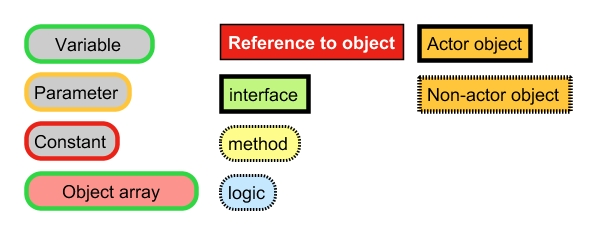
\includegraphics[width=0.75\columnwidth]{ChapterFramework/figures/Obj_key}%
%\includegraphics[width=0.85\columnwidth]{ChapterModels/Figures/hillclimbExcel}%
\caption{Key for model framework diagrams}%
\label{fig:frameworkKey}%
\end{figure}

%%%%%%%%%%%%%%%%%%%%%%%%%%%%%%%%%
Consider a Person, labelled $a$, who is looking for a firm $f$ offering the best wage. Actors all have location, so let the distance between them be $af$. If people have to `commute' to their work place, the time taken to commute is zero sum with the time they can put into working. Here, a `commute' is taken to be twice $af$. The upper distance limit on whether a firm enters into $a$'s considerations has to be less than $a$'s one available day in total - half a day there, half back - otherwise there is no time left at all to contribute to production. So $f$ can only be a maximum of half a day away. If $c_{af}$ is the commute time between them then -

\[
c_{af}=2\cdot t_{af}\]

The set of potential employers for a Person is thus immediately limited by commute distance. This set of potential employers is labelled as $PE_{a}=\{f_{n}...\}$ It can contain any number of firms within commute range. The set of firms is just  $F=\{f_{1},f_{2},...,f_{n}\}$ So, $p$ uses the following to populate $PE_{a}$:

\[
for\, each\, f_{n}\in F\]

\[
if(c_{af(n)}<1)\, then\, f_{n}\in PE_{a}\label{eq:circlerule}\]

Which translates as: unless the time it takes for $a$ to get to $f_{n}$ and back again (the commute distance) is more than one, add it to my set of potential employers. This guarantees there is time left for working, and $a$ can then use it to see if working is worthwhile. 

%This varies between model types, but what all models share is that people's wage will be proportional to the time they can contribute. In the simplest, the `wage' is a single good: the direct product of $a$'s contributed labour. 
So what is a `best wage?' If firms are paying in money, this is the maximum amount a person can get, having accounted for any commute loss. 

So $a$'s actual wage is:

\[
w_{a}=W_{f}\cdot l_{a}\]

This creates a new set: a list of wages from $PE_{a}$:

\[
Wagelist_{a} = 
\]

Whether paid in raw goods or money, what this means is that, for the set of potential employers, $PE_{a}$, there is always one objectively best wage, since distance cost has been accounted for. It also mean that, if wages are the same for all firms, the nearest firm offers the best wage.

So $a$ selects the one firm with the maximum wage and adds it to the Bundle:

$bestwage = max{}$

\cmt{blah! Do I really need to be going to these lengths just to say `select firm with best wage, accounting for commute costs?' Must be a more succinct way!}

%Depending on the model, people may be able to choose between working and backyard production. Backyard production is linear: if people are producing for themselves, time can be converted directly into goods. 
%In this case, $t$ is literally the budget: $u$ can be maximised with a budget of $x+y=t=1$. Space does not enter into this decision: by definition, backyard production means staying put.

%Consider a generic utility function with two goods: $u=f(x,y)$. The `budget' a person has to work with is, at base, one day or $t=1$. However, $t$ needs converting into goods before a utility value can be found. Depending on the model, matters are complicated because $t$ can be converted into either goods or money first - via a wage - and then to goods. But what about working?

%The most complicated set of steps a person will have to take involves earning a money wage and then seeking to buy goods with that wage. People know nothing about any firm's productivity. They only know the wages and goods prices they find, and their own utility function. So a person cannot know what quantity of goods they can get without first knowing a wage and goods prices. 

%%%%%%%%%%%%%%%

%The method used is a stochastic search: budget `slices' are randomly allotted to each good and then adjusted towards better mixes (see the code appendix and comments within the classes themselves for full details.) 
%To do this, the best wage is split into randomly sized `slices' of money and whatever quantity of goods that would buy is 
%that gets us. Or we don't if stock is out: we try to reallocate, until either all stock is gone or all money is gone. That seems easier explained in words than in anything else. Hmm.
...
Section x explained that a `general' analysis aims to include all factors affecting economic outcomes, because the full set of inter-relations may lead to very different outcomes from just looking at a partial picture. However, it was also argued [Isard etc] that such general analyses are made even more complex when space and agents become involved. Coordination issues abound, and space itself does away with the indispensable simplifying assumption of a single clearing market. This section goes into more depth, explaining exactly what this means for the modelling choices made in the thesis.
The main goal of the model framework is to provide methods for easily comparing different spatial economic scenarios. To do this, it needs to be able to deal with a large number of different options. The range of these options is potentially confusing; this chapter aims to reduce that confusion to a minimum by clearly laying out a reference guide to the available options. It also explains how a particular option-set (a `scenario') is described when model results are presented.
...
Space bits
%Probably need to explain how it affects discrete outcomes somewhere

%In the models that use explicit space, distance measurement is built around the idea of one Person's `day'. The distance a Person can get in one day serves as one unit. That distance Actors can get in one day may change over a model run, but it still stands as a base for comparison in that run. Distances will be described this way:

%Moved to space costs chapter

%As discussed in section \ref{sec:spacechange}, any factor that can be used to `buy movement' will be labelled an \gls{mbf}: units of distance can be bought with it. Depending on the type of actor, specific \gls{mbf}s \emph{must} be spent to cover distance. The most obvious \gls{mbf} is time: it takes a certain quantity of time to cover a given distance. For the sake of readability, `units of distance' will be referred to as `miles': these are entirely abstract, and are used purely to make description more readable (`miles per day' rather than `distance units per day'.) A factor can be an \gls{mbf} as well as a standard productive factor entering into a firm's production function. Again, time fits this description: where People are not putting time into moving, they can put it into production. Often, economic models use the term `labour' to refer to this productive factor; in the core model, it is the only factor. In more detail:

%\begin{itemize}
%\item For each model day, each actor is given $t=1$ to spend: in other words, they have `one day per day' and will aim to make optimum use of it. (See note below for more on this.)
%\item A given distance between $r$ and $s$ will be labelled $rs$. The time is takes to cover it is $t_{rs}$. So, generically, $t_{rs}=f(rs,tech)$, where $tech$ is some technology that has an impact on the time taken. For many of the models, time to cover a given distance will be a function of the distance alone. However, the generic factor $tech$ here indicates that the amount of time to cover a distance may change. 
%\item $tech$'s role in this function is separate from its cost. For example, if $t{}_{rs}=rs/tech$, the time taken to travel between $r$ and $s$ goes down as the level of $tech$ increases. It says nothing about $tech$'s cost. Indeed, from the point of view of actors, it could be free and ubiquitous.
%\end{itemize}

%q: what's the average distance between randomised actors in a one-width world? Well: of course, it drops as more actors are added. Oooh - that's interesting! Didn't think of that before! If I want to control distance between actors, that needs fixing!

%What other values do I need to discuss? How to measure changes in clustering, thus agglomeration. What units? And for good movement cost, which we'll call delivery cost. Actually, I'm not sure how I've defined that! It has to be large because of the small size of the world, of course, if it's to have an impact.
%Then there's: wages, good price etc.
This choice of spatial measurement impacts on how space costs must be set. Many of the models use a `delivery cost' for goods (see section x below for full details.) In a world that is only one or two units wide, and where actors may be clustered together in a small part of that space, good movement costs must be proportionately higher to have any economic impact.
...
The total price of a good includes the cost of moving it across space. Consider a good $g$. The total price is $P_g$, and consists of three parts: $p_g$, the base price; $c$, the cost to move one unit of the good across one unit of distance; and $d$, the distance itself. So in full:

\begin{equation}
P_g = p_g + (c \cdot d)
\label{eq:totalgoodcost}
\end{equation}

If $c = 0$, then, the good will cost the same anywhere in space. If $d = 0$, a Person is at the same location that the good is being sold from and, again, only has to pay the base price $p_g$. The variable $c$ is the simplest way possible to represent the cost of moving goods across space. The fact that it is the cost per unit of distance means it can stand in for weight. Section \ref{sec:explorechangingcosts} works through the mathematical implications of this.
%The thesis models are abstract: they are not calibrated to any particular real-world situation. As far as possible, then, values are normalised to keep analysis and presentation as clear as possible. That said, it is still worth discussing the way numbers are set up in the model.
%In defining parameters, some concepts from object-oriented programming are borrowed. Variable parameters can vary at any time in or between model runs. Static parameters are fixed for single model runs, but may vary between runs if, for instance, they are subject to a parameter sweep or randomisation. Final parameters never change. Where appropriate, a description will also be given of the exact way in which parameters change. Most commonly, this will be whether wages, prices, stock and money are fixed and if not, how they are set. 
...
Lastly, the nominal value of wage and good price matters less than their ratio: what a Person can buy with their wage. This is the `real wage'. 
..
\subsubsection{Getting a set of Goods} 

A Bundle will contain a list of all goods, either within a given range or for the whole model space. Each good is represented by a `Good' object that contains the following:

\begin{itemize}
	\item Cost per unit, including delivery cost.  
	\item Reference to the Firm selling the good.
\end{itemize}

As regards good delivery costs, there are various ways of calculating this. See section x \cmt{Section for outlining approaches to pricing goods across space} for full details, but an example illustrates the principle. If a firm has a base unit price $p$ and a delivery cost to move one unit for one `mile' $d_{p}$, and the distance to deliver is $af$, then the cost per unit can be set to $p + (p\cdot d_{p}\cdot af)$. This is the value stored in the Good object. The fact that a space cost is part of that is hidden to the Person: they make their decision based entirely on this single calculated cost.
\cmt{That's described above I think}
%Aside from that, the output could be physically less, physically more. Generally it would need to be worth more to be economically feasible, but that doesn't logically have to be the case: people could be coating electronics in marmite, thus ruining it and making it heavier.
%Looking at LoV, the same outcome occurs - pretty much:
%Point of trade is where the \gls{increts} are
%No extra physical output, pure increase in value. Pretty much costless: value comes about purely through exchange. Cheapest value creation possible. (Though not free since it needs to be got to market.)
....
\subsection{Misc}

\cmt{Very rough draft follows. Keeping in.}

Why the above choices? Quick blarb. Firstly, utility is the one element from analytics this thesis prioritises. It is the micro-economic foundation of \gls{ge}, and I want to see what the consequences are for a) keeping it and b) putting it in an agent context. So the above setup allows people to optimise their utility based on a function like love of variety - taking any number of goods. There is plenty of criticism to be made. Some of those:

How is it realistic for people to `sample' different spatial locations for their Bundles?

How it it realistic for people to know the price of all goods within a certain range, without expending any cost to get that information?

Same for the optimisation algorithm itself: putting an arbitrary number of goods through many steps to produce a single utility level. How is that cognitively realistic?

Answer: it isn't. We have to be open and strategic about the things that aren't realistic. My aim is to use micro-economics and see what the results are. I have to argue about how I can locate that in reality. How can People realistically acquire knowledge of all goods in an area in order to calculate utility from a \gls{loveofvariety} function? Put that way it seems unrealistic. But it may stand in well enough for reality...

Firms have a very different decision structure to people: feedback over time using only internal data versus instant decision making from collected data. So Firms and People are active and passive in different ways. Firms can change their prices; People must accept the prices they face and optimise accordingly. People can quiz their surroundings to collect data and act immediately; Firms are forced to blindly attempt an action and wait to discover the consequences. 

Firms could be given knowledge of the distance of People working for them or buying from them. Would this help? It's one of the things I need to work on: can actors be given enough information to produce stable, economically sensible outcomes?

This distinction is a consequence of the particular approach to utility used as the foundation of the modelling approach. (As discussed... where?) In contrast to \gls{ge} and Fowler's agent approach, no `objective' demand levels are available to the firm. They can only interpret the data they receive as the market changes. They could potentially be allowed to carry out `market research': quizzing People about what they emph{would} buy given infinite stock levels. 
..
Ultimately, the model structure itself cannot do all the work of showing its relation to reality. There are very few solid rules about how to build a model that can claim to map to the real-world features the modeller is interested in. The modeller must make an argument, with as much clear awareness of the limitations of the method as possible. Section x works through a specific example of this issue, looking at two different ways to approach \gls{increts} in an agent model, and how these impact on agent timing issues.
\cmt{section x: production and timing}

The `meaning' in data, meaning response is one example. This sort of thinking tool may be more useful than any number of coding structures. So again, the isomorphism between code and theory may also be implicit, rather than hard-coded.
..
\subsection{Basic timing choices}

There are two different uses of the concept of `time' in the model: it is important to be clear on the difference between them. A `day' is the most fundamental unit of time, but it is used in two different ways in the model:
\begin{itemize}
\item `Day' as a measure of distance: the time it takes for an actor to move across a given distance of space. 
	\item 'Day' as a model iteration - so actually the passage of time for actors in the model. The easiest way to avoid confusion here is to use the term `iteration' when discussing model run days.
\end{itemize}

`Day as distance' was discussed in section \ref{sec:peoplemoving}. The next section discusses model iterations.
..
%Taken from field diary, 'problems for later'. This is probably better for the intro.
To what extent do these coordination problems need solving before a full picture of spatial economics can be formed? Can these coordination issues be avoided by looking instead at partial analyses, while still saying something useful about spatial economics? Or does the coordination problems need solving before this can be known?
..
Of most importance is the fact that many partial models are used. This means fixing the majority of the model parameters to focus on one particular feature of interest. This makes for very different models. Consider the type of model Fowler presents (see section x): a number of Firms and People attempt to optimise revenue and utility respectively. Firms have economies of scale, wages are paid and goods have a cost. 
Any attempt to make this decision simultaneously will be 
Can I do an example with two Firms? Oh, prob easier with the three-actor BY problem.
..

Options involving making decisions at different timepoints present actors with two possibilities, both having their own problems. Looking at it from an actor's point of view:

\begin{itemize}
\item If I add myself, and calculate output based on who was there before me, they do not gain from the extra \gls{eos}, even though I do.
\item If I add myself and wait until the end of the day to work out my productivity, the basis for my decision will probably have changed, since others may have contributed.
\end{itemize}

Whichever of these an actor chooses - decide now, or wait and see - the basis on which others made their decision will be altered. This is not necessarily a problem, if the contributed input is considered as a flow that takes place between actor decision points. This is intuitvely plausible: an actor decides who to work for, and can be considered `working' until it is their turn again.

Have I just convinced myself that it's a good idea? What's the problem then? Well, that they get all their output in one go. Not to mention, negative stock? Well hey, why not?
%(It will be shown, for example, that completely unrealistic market behaviours can be the consequence of poor decision-ordering code.)
%There is, however, a modelling ``trick'' used to avoid the need for strategic decision-making. To understand why this is necessary, consider the ``El Farol Bar problem.'' 
%Decision ordering then, occurs during one `day', is randomised, and instantly updates productivity information. Later, other options for decision ordering will be discussed, in order to test what difference they may make to outcomes. For now, there are no expectations, no memory, and thus no strategic choices to be made: each time an actor looks at the world they decide anew. When they next make their choice, a different set of actors may have left or joined the site they previously chose.
%The output they get is based on what happens \emph{at that moment}. This may mean slight adjustments to output could have changed their decisions, but the effect should be slight. 
%But every time someone makes a decision, they may decide to move elsewhere. Also, if an actor does choose a collaborator, they have just changed the output for whoever had already worked there. From an actor's point of view, the dilemma they face is - 
...
It might seem the better option, then. Proponents of more analytic approaches might say this was just the sort of detail that illustrates why agent modelling is best avoided. That may be so, but it does present some interesting questions: what does the choice of either production function imply, if anything? In the example above, what does it mean that a rational actor - albeit one with no expectations or ability to judge their decisions over multiple timesteps - fails where a randomised actor can succeed?

Add: this problem does not just relate to the need to `bootstrap', but it also presents itself if Actors are attempting to adjust values on subsequent timesteps. I'm thinking of smooth function working in LoV single actor....

Revolving around: bug or feature? Arbitrariness of assumptions, and what they're meant to achieve. 

\cmt{bug or feature? Where do I discuss that? Also, how to describe timing issue of e.g. changing time input between Firm actions? And online vs offline optimisation? That relates to timing but overlaps with action. Relates also to whether actors are facing a `static' world or not... how to tie that together coherently?}
%WUD 40	Blind search agents: advantage = they have no need to know everything at the same time. Attempts to improve position can be separated out over many timesteps.
%WUD 43	Brute force vs analytic optimisation: catch 22 in actor model where they try to optimise on their time-step: no stock = no point in working; no work = no stock.
%This production function must meet two needs: to be capable of defining a smooth transition from backyard production, and offer a way to avoid a fixed labour requirement. Backyard production is defined for a single actor only: input of time is directly turned into output of goods linearly for that actor; this linear output makes `space impossible' and actors never have the incentive to move or collaborate. \gls{increts} come into play where time input is more than one day in total. 
%However, there are some issues when using this in an agent-based context. A full discussion of these can be found in section \ref{sec:agenttimings}; briefly, the fixed labour requirement presents an obstacle to actors `bootstrapping' a model run, and defining Firm outcomes in terms of an abstract `total labour requirement' is problematic.
%\cmt{ref to core model discussing inc rets: where is that now? Still exists?}
%Different kinds of uncertainty: that one is physical. The measurement is accurate. My agents: having to react to other agents, not knowing how they will respond...?
%stick the hayek stuff in here: price as a signal cannot be reduced to something simple. It's the end of a process, a summation of carefully won, specialised knowledge: metis.
\cmt{meaning: rarely defined explicitly? I'll probably end up defining it completely implicitly. If so, come back here and change `rarely' to `never in the models presented here.' Also, I think this issue is discussed in this chapter, and belongs here.}
The slippiest term here is `meaning'. As will be discussed in chapter \ref{chapter:models}, meaning is rarely defined in explicit code form. Rather, the overall code structure is taken to represent meaning for a particular agent. 
In-keeping with the overall aim of using as simple assumptions as possible, meaning will be used as narrowly as possible. For example, it is possible for cultural meaning to vary geographically, in economically vital ways.
This kind of `cultural economic' meaning will be excluded: data will use the same units and have the same metadata assumptions for all actors. 
As in Jacobs, the \gls{dmr} framework should be considered a feedback loop. When considered as a feedback, the simplest form of meaning becomes apparent. An actor takes an action, waits to receive data, and then interprets that data based on that action before responding again. 
While computers are iterative by default (the system clock imposes a discrete structure), this does not necessarily mean that agent models \emp{must} be discrete, or indeed that they must be algorithmic: approximations to continuous and algebraic\footnote{Symbolic computing is capable of producing good analytic results: for example, where iterative approaches to integration like Runge Kutta functions can only approximate, symbolic computing can generally do as well as analytics in producing exact results where they exist.} functions are possible. \gls{abm}, however, has tended to integrate discrete time-steps into its approach, and methods are employed to design agent models with appropriate timing. 
..
The most important difference between model types is those that attempt some element of feedback, where a flow of stock or money is cycled over many timesteps.
No it's not: I can make the model general with stock `perishing'. 
The Firms generally do not get the delivery cost: it `melts away'. Should mention: any money circulation model has problems with that.
..
If one set of Actors is able to make objectively optimal decisions `instantaneously', presuming everything to be static, the other set cannot. 
Is that true? Is a Firm not able to make an optimal location choice? Not without knowing what revenue would be for certain points - and it cannot do that without getting a record of all People's inputs. 
Well, I can see a way they could, in parallel fashion. 
For a Firm to manage the same style of `sampling' as People do, where several random location point `Bundles' are compared, they would need to know the exact demand from all People at those points. The model could do this, in principle, but it would mean requiring all People to re-calculate their utility levels for each sample. 
In effect, of course, this does happen: the difference is that Firms do this optimisation `online' over a number of timesteps.
Both wages and good cost are set by `the market', which for an agent model must come about through either distributed decision-making, or otherwise some artificial construct to circumvent the coordination problem, like an auctioneer or, for the labour market, an assumption of collective bargaining. [Marc Oeffner]
\subsection{Action, timing and co-ordination \label{sec:actions}}
..
Points to make: utility is offline, DMR is online, transmission belt online, spatial eq online.
Also: modeller may be interested in a process as an `optimisation' that one doesn't assume actors should know about. This is the case with thinking about model-wide welfare: the overall optimisation is `online' in the sense that it results from actor interaction, but the actors themselves are only attempting to improve their own situation, knowing nothing about the global picture.
As argued above, it is tempting to mistake an agent model for a direct isomorph of reality. But is it necessary to either represent an entire population as individual agents, or give up and use some other method instead like a gravity model, if it can be shown that the exact number matters less than the dynamics produced? Agent models of any number can be normalised just as analytic models can, with all the same caveats and checks involved in doing that.
\cmt{In the thesis, I'd probably need an example of this. E.g. the effect on prices being the most obvious. Under what circumstances could one ignore it?}
..
Stick in Brakman's analysis of when Firm numbers affect competition and why `assuming a large number' then allows other things. And why I'm arguing that's fine for ABM: say `assume a large number' does not mean you have to HAVE a large number. If you are interested in: stochastic results, interaction / emergence results, the number you need for that can be different from e.g. comparing to the Brakman example the number you need for being able to assume competition effects are small. 
..
Number of agents can have different impacts. Some of those effects you may be interested in, and others you won't. Example of competition effects, which are different for `very large numbers'. 

So, x-ref to that section.

Different uses and impacts of `number'; connects to representative agent, and so micro and macro.

%Friedman needs to come in here! Is this a little early in the chapter? I should cover broader view of ABM at this point.
%I've found lots of quote about this, I should gather them here really.
Can fix certain prices while allowing e.g. location competition. But note the arg is based on `assuming large numbers' and that these are all kept exogenous to the model. This would be the case if, for example, fuel prices are fixed exogenously: modelled Firms are presumed to have no effect on them. This is not an unreasonable assumption.
%since it keeps things as simple as possible. If space wraps (either a `racetrack' or torus world), it must be large enough to make sure actors' spatial search does not overlap itself. For example, if an actor can travel for `one day', their full search circumference spans two days, and the size of the space they are in must be at least this large. 

Section \ref{sec:spacecostgoods} explained the simple equations used to set the cost of goods, and that the cost of moving people can be framed in the same way. 

Come back - how to tie to choosing best wage below?

\end{comment}


